\documentclass[12pt,a4paper]{report}
\usepackage[utf8]{inputenc}
\usepackage[french]{babel}
\usepackage{tikz}
\usepackage{listings}
\usepackage{amsmath}
\usepackage{amsfonts}
\usepackage[T1]{fontenc}
\usepackage{amssymb}
\usepackage{graphicx}
\usepackage{color} 
\usepackage{fancybox}
\usepackage{biblatex}
\usepackage{lmodern}
\usepackage{tikz}
\usepackage{relsize}
\usepackage{float}
\usepackage{caption}
\usepackage{subcaption}
\usepackage{arabtex}
\usepackage{utf8}
\usepackage{pgfplots}
\usepackage{algorithmicx}
\usepackage{algpseudocode}
\usepackage{wrapfig}
\usepackage{tikz}
\usepackage{listings}
\usepackage{xcolor}
\usetikzlibrary{shadows}
\algdef{SE}[DOWHILE]{Do}{doWhile}{\algorithmicdo}[1]{\algorithmicwhile\ #1}%
\usepackage{comment}
\usepackage{lipsum}
\usepackage[ruled,vlined, french, onelanguage]{algorithm2e}
\usepackage{fancyhdr}
\usepackage{hyperref}
\usepackage{fancybox}
\usepackage[left=3cm, right=3cm, top=3.00cm, bottom=3.5cm]{geometry}
\usepackage{mdframed}
\usepackage[Glenn]{fncychap}
\graphicspath{{./figures/}}
\renewcommand{\baselinestretch}{1.2}
\graphicspath{{figures/}}
% Configuration du style du code
\lstset{
    language=Python, % Langage du code
    basicstyle=\small\ttfamily, % Style de base
    keywordstyle=\color{blue}, % Couleur des mots-clés
    commentstyle=\color{green!40!black}, % Couleur des commentaires
    stringstyle=\color{orange}, % Couleur des chaînes de caractères
    breaklines=true, % Activation du retour à la ligne automatique
    numbers=left, % Affichage des numéros de ligne
    numberstyle=\tiny\color{gray}, % Style des numéros de ligne
    stepnumber=1, % Intervalle entre deux numéros de ligne
    showstringspaces=false, % Ne pas afficher les espaces dans les chaînes de caractères
    frame=single, % Affichage d'un cadre autour du code
    backgroundcolor=\color{gray!10}, % Couleur de fond
    captionpos=b % Position de la légende
}
\begin{document}
\begin{center}
\thispagestyle{empty}
\rule{1\textwidth}{0,5pt}\vspace{0,5cm}\\
\textbf{Université de montpellier\\
Faculté des sciences}\\
\vspace{1cm}
\begin{figure}[H]
    \centering
    
\includegraphics[width=0.3\linewidth]{logo universite de montpellier .png}
 
   
\end{figure}

\end{center}

\begin{center}
\textbf{Département mathématique}
\vspace{1cm}
\hspace{2cm}\\
\textbf{\huge{TP3 }} \\
\vspace{1cm}
\textbf{M2 MIND-SIAD}
\vspace{1cm}

\rule{0,9\textwidth}{3pt}\\
\vspace{0,3cm}
\large\textit{\textbf{ Support Vector Machine (SVM)}}
\normalsize
\rule{0,9\textwidth}{3pt}\\ 
 
\end{center}
\vspace{1cm}
\hspace{0,2cm}
\begin{center}
\textbf{Réalisé par} :\\ Lamia Oulebsir\\Naima Radouan
\end{center}
\\
\vspace{1cm}
\begin{center}
\textbf{Septembre 2025 }
\end{center}
\pagestyle{plain}




\tableofcontents
%\newpage

\section{Introduction}
%\addcontentsline{toc}{chapter}{Introduction}

Les machines à vecteurs de support (SVM) constituent des méthodes de classification supervisée largement utilisées, notamment pour leur efficacité à résoudre des problèmes de classification binaire en séparant les données grâce à des hyperplans optimaux. Ce TP a pour objectif d’implémenter et d’évaluer des modèles SVM dans différents contextes, en examinant l’effet des types de noyaux, des paramètres de régularisation, de l’ajout de variables parasites, ainsi que l’amélioration des performances via une réduction de dimension par PCA.

\section{Principes Généraux et Fondements Mathématiques des SVM}


Les \textit{Support Vector Machines} (SVM), introduites par Vladimir Vapnik dans les années 1990, sont des outils destinés à résoudre des problèmes de classification binaire. Leur principe repose sur la recherche d’un hyperplan affine séparant au mieux les données de deux classes distinctes, tout en maximisant la marge entre elles. L’hyperplan optimal est celui qui maximise la distance minimale avec les points les plus proches de chaque classe, appelés vecteurs de support.

\subsection{Classification binaire supervisée}

Considérons un ensemble de données composé d’observations \( x = (x_1, ..., x_p) \in X \subset \mathbb{R}^p \) associées à des étiquettes \( y \in \{-1, 1\} \). Dans ce cadre, l’objectif est de déterminer une fonction \( \hat{f} : X \to \{-1, 1\} \) capable de prédire l’étiquette d’une nouvelle observation en fonction de sa position relative à l’hyperplan séparateur.

L’hyperplan affine est défini par l’équation \( \langle w, x \rangle + w_0 = 0 \), où \( w \in \mathbb{R}^p \) représente le vecteur normal à l’hyperplan et \( w_0 \) le biais. La règle de décision est donnée par :
\[
\hat{f}(x) = \text{sign}\left(\langle w, x \rangle + w_0\right),
\]
de sorte que la prédiction de l’étiquette soit \( +1 \) si \( \hat{f}(x) > 0 \) et \( -1 \) sinon.

\subsection{SVM dans des espaces de grande dimension}

Lorsque les données ne sont pas linéairement séparables dans l’espace d’origine \( X \), les SVM appliquent une transformation non linéaire \( \Phi \) projetant les données dans un espace de dimension supérieure, appelé espace de caractéristiques (ou espace de Hilbert \( H \)). L’objectif est de rendre les classes séparables linéairement dans cet espace.

Comme le calcul explicite de cette transformation peut être coûteux, les SVM utilisent le \textit{kernel trick} permettant de calculer directement les produits scalaires dans l’espace transformé :
\[
K(x, x') = \langle \Phi(x), \Phi(x') \rangle.
\]
Parmi les noyaux courants, on trouve :
\begin{itemize}
    \item \textbf{Noyau linéaire} : \( K(x, x') = \langle x, x' \rangle \),
    \item \textbf{Noyau RBF gaussien} : \( K(x, x') = \exp(-\gamma \| x - x' \|^2) \),
    \item \textbf{Noyau polynomial} : \( K(x, x') = (\alpha \langle x, x' \rangle + \beta)^\delta \).
\end{itemize}

\subsection{Formulation du problème d’optimisation}

Le SVM vise à maximiser la marge entre les classes tout en limitant l’erreur de classification, ce qui se traduit par le problème suivant :
\[
\min_{w, w_0, \xi} \left( \frac{1}{2} \| w \|^2 + C \sum_{i=1}^n \xi_i \right),
\]
sous les contraintes \( \xi_i \geq 0 \) et \( y_i (\langle w, \Phi(x_i) \rangle + w_0) \geq 1 - \xi_i \) pour tout \( i \).

La solution optimale s’exprime en fonction des vecteurs de support \( x_i \), c’est-à-dire les points pour lesquels les contraintes sont actives (\( \alpha_i \neq 0 \) dans la formulation duale). Les paramètres \( w \) et \( w_0 \) sont déterminés en résolvant un problème d’optimisation quadratique avec contraintes linéaires.

\subsection{Contrôle de la complexité et régularisation}

Le paramètre \( C \) permet de contrôler la complexité du modèle : une valeur élevée réduit les erreurs de classification mais peut provoquer un surapprentissage, tandis qu’une valeur faible favorise la généralisation en tolérant certaines erreurs.  

Une alternative est la \(\nu\)-classification, qui ajuste la proportion de vecteurs de support dans l’ensemble d’apprentissage via un paramètre \( \nu \in [0, 1] \).

\subsection{Extension aux problèmes multi-classes}

Pour des problèmes multi-classes (\( Y \in \{1, ..., K\} \)), les stratégies les plus utilisées sont :
\begin{itemize}
    \item \textbf{Un contre un} : construire un classifieur pour chaque paire de classes (\( K(K-1)/2 \) classifieurs),
    \item \textbf{Un contre tous} : construire un classifieur pour chaque classe \( k \), séparant les données où \( Y = k \) des autres.
\end{itemize}
\section{SVM sur le Dataset Iris}

Dans cette première partie, nous utilisons la bibliothèque \texttt{scikit-learn} pour implémenter les \textit{Support Vector Machines} (SVM). Le dataset \texttt{Iris} contient trois classes de fleurs : Setosa, Versicolor et Virginica. Nous avons restreint cette étude à une classification binaire, en ne considérant que les deux premières classes (Setosa et Versicolor) et les deux premières variables. Le but est de comparer la performance d’un SVM avec noyau linéaire et un SVM avec noyau polynomial.


\subsection{chargement des données}

Nous avons commencé par charger le jeu de données Iris et appliquer une normalisation pour centrer et réduire les données, à l'aide de la classe \texttt{StandardScaler}. Ensuite, nous avons filtré les observations pour ne garder que les deux premières classes et les deux premières variables. Une division des données en ensembles d'entraînement (50 \%) et de test (50 \%) a été effectuée pour évaluer les modèles.

\begin{lstlisting}[language=Python, caption=Chargement des donnees et pretraitement]
# Charger les données Iris
iris = datasets.load_iris()
X = iris.data
scaler = StandardScaler()  # Normalisation des donnees
X = scaler.fit_transform(X)
y = iris.target
# Filtrer pour garder uniquement les classes 1 et 2 et les deux premieres variables
X = X[y != 0, :2]
y = y[y != 0]
\end{lstlisting}

\subsection{Division des données en sous ensemble(entraînement et test)}

Nous avons divisé les données en 2, 50\% pour l’entraînement et 50\% pour le test.
\begin{lstlisting}
X, y = shuffle(X, y, random_state=42)
X_train, X_test, y_train, y_test = train_test_split(X, y, test_size=0.5, random_state=42)
\end{lstlisting}

\subsection{ Classification de la classe 1 contre la classe2 du Dataset Iris avec un noyau linéaire}

Nous avons commencé par implémenter un SVM avec un noyau linéaire, et nous avons utilisé la grille de recherche qui permet de tester différentes valeurs de C sur une échelle logarithmique.
\begin{lstlisting}
parameters = {'kernel': ['linear'], 'C': list(np.logspace(-3, 3, 200))}
clf_linear = GridSearchCV(SVC(), parameters, cv=5)
clf_linear.fit(X_train, y_train)
#  Afficher le meilleur parametre C et la precision
print('Meilleur parametre C pour le noyau linéaire :', clf_linear.best_params_)
\end{lstlisting}
Nous obtenons comme meilleur paramètre C pour le noyau linéaire une valeur : 0.297, ceci indique que le SVM linéaire tolère certaines erreurs pour tracer une frontière simple et stable. Le modèle avec un noyau linéaire obtient une précision de 66 \% à la fois sur les données d’entraînement et sur les données de test, cela signifie que le modèle généralise correctement, il ne présente pas de surapprentissage ni de sous-apprentissage.

\subsection{ Classification de la classe 1 contre la classe2 du Dataset Iris avec un noyau polynomiale}

Nous avons utilisé un SVM avec un noyau polynomial, nous avons testé différentes
 valeurs du degré du polynôme, ainsi que du paramètre C et $\gamma$ 
 \begin{lstlisting}
Cs = list(np.logspace(-3, 3, 5))
gammas = 10. ** np.arange(1, 2)
degrees = np.r_[1, 2, 3]

# Entraîner le modele et selectionner le meilleur ensemble d'hyperparamdetres
parameters = {'kernel': ['poly'], 'C': Cs, 'gamma': gammas, 'degree': degrees}

clf_poly = GridSearchCV(SVC(), parameters, cv=5)
clf_poly.fit(X_train, y_train)
# 

print(clf_poly.best_params_)
print('Generalization score for polynomial kernel : %s, %s' %
      (clf_poly.score(X_train, y_train),
       clf_poly.score(X_test, y_test)))

\end{lstlisting}
\begin{itemize}
\item Nous obtenons comme meilleur valeur de C : 0,032,  ce qui suggère que le modèle tolère plus d’erreurs dans les données d’entraînement, cette valeur permet au modèle de géneraliser mais il risque de sous-apprendre si les données sont bien séparées. 
\item le noyau polynomiale a choisi un modèle linéaire simple((degré 1, C petit), Cela suggère que le noyau polynomial n’a pas trouvé de relations non linéaires significatives dans les données.
\item $\gamma = 10$ le parametre  contrôle l’influence d’un seul point d’entraînement. Un $\gamma$ élevé (comme ici, 10.0) indique que le modèle considère les points proches de la frontière de décision de manière plus importante, ce qui peut potentiellement créer des frontières plus complexes.
\end{itemize}
\begin{lstlisting}
Generalization score for polynomial kernel: 0.66, 0.66
\end{lstlisting}
 Les scores de généralisation montrent que le modèle polynomial obtient une précision de 66\% sur l’ensemble d’entraînement et aussi l'ensemble de test, ce qui indique qu'il n'y a pas de sur-apprentissage, cela suggère une généralisation cohérente mais modérée. L’augmentation de la complexité du noyau n’améliore pas beaucoup les performances.  
 \newpage 
 
\subsection{ Visualisations }

Les figures ci-dessous montrent les données projetées dans l'espace bidimensionnel ainsi que les frontières séparatrices.
\begin{figure}[H]
    \centering
    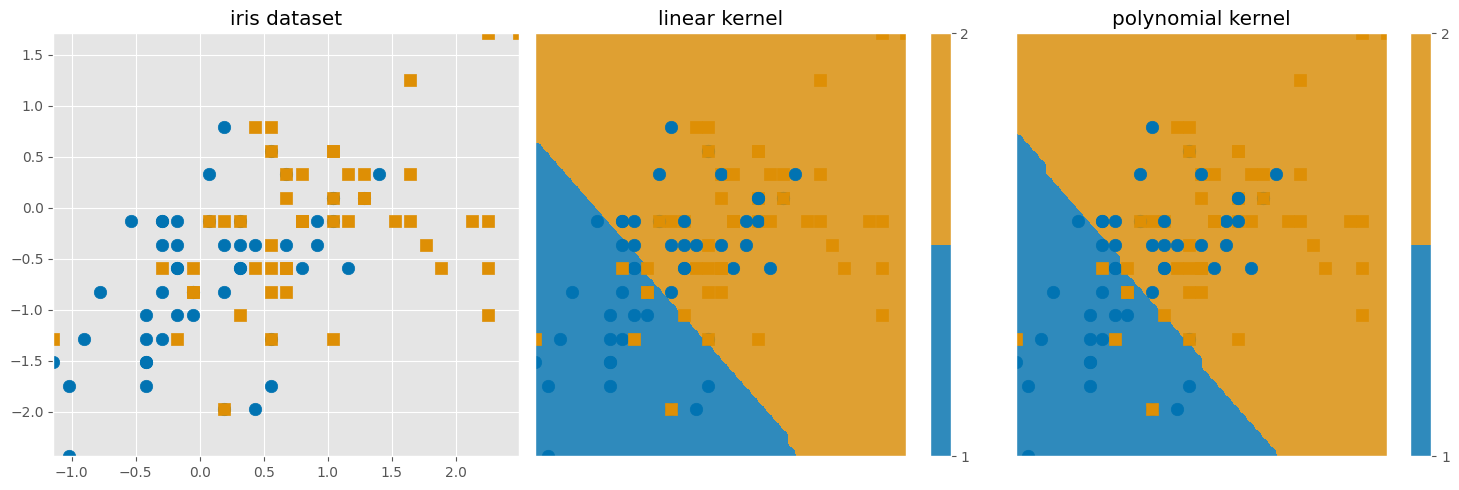
\includegraphics[width=1\linewidth]{images/iris.png}
    \caption{ Classifications avec noyaux linéaire et polynomial (degré 1)}
    \label{fig:placeholder}
\end{figure}
Le noyau polynomial avec degré 1 produit une frontière de décision quasi linéaire, qui sépare assez bien les deux classes. Les scores (66 \% sur train et test) indiquent une performance correcte et une bonne généralisation(pas de sous-apprentissage ni de sur-apprentissage).
\begin{figure}[H]
    \centering
    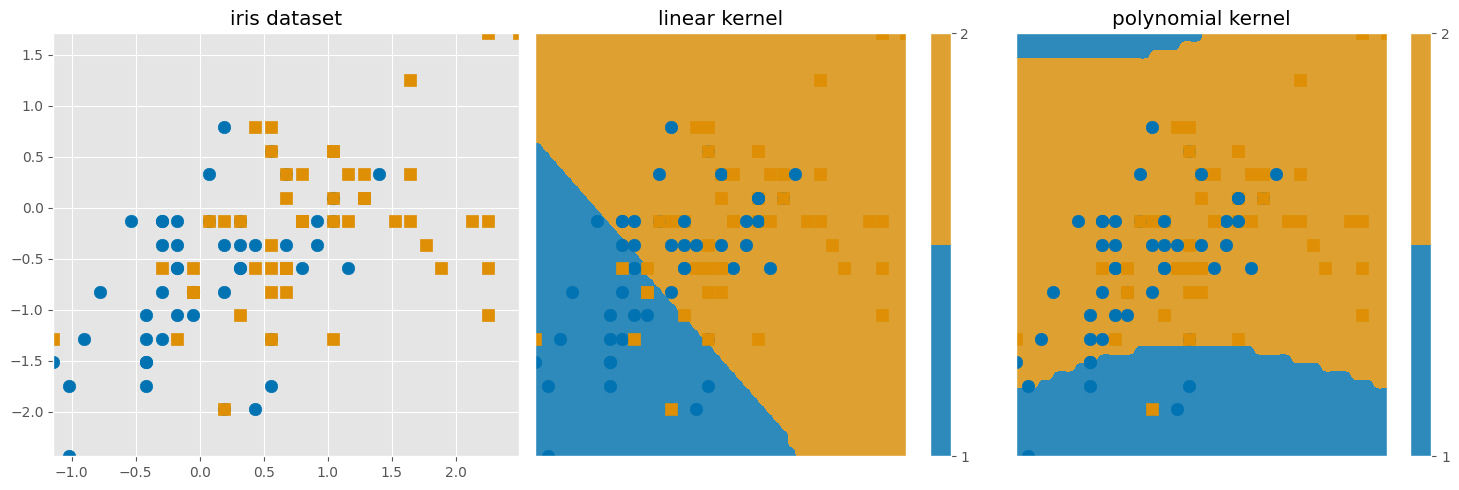
\includegraphics[width=1\linewidth]{images/results_deg2.png}
    \caption{Classifications avec noyaux linéaire et polynomial (degré 2)}
    \label{fig:placeholder}
\end{figure}
L’image de droite montre la frontière de décision obtenue avec un SVM à noyau polynomial de degré 2 (C=0.001, gamma=10). On voit que la frontière est plus courbe et complexe que celle du noyau linéaire, mais le modèle n’arrive pas à bien séparer les deux classes. Cela se traduit par un score de 0.64 sur l’entraînement et seulement 0.44 sur le test, indiquant que le modèle sous-apprend : il tolère trop d’erreurs (C très petit) et généralise mal aux nouvelles données.\\
-  Le modèle avec un noyau linéaire (degré 1) et C = 0,031 obtient de meilleurs scores sur les deux ensembles, cela suggère qu’une séparation linéaire est plus appropriée pour ce problème.

\subsection{Impact de Noyau linéaire et du paramètre C sur un jeu déséquilibré}

Dans cette partie, nous avons utilisé le script \textbf{svm\_gui.py} 
afin de générer un 
jeu de données fortement déséquilibré, caractérisé par une répartition où une classe 
concentre environ 90\% des observations contre seulement 10\% pour l’autre. 
L’ajustement du paramètre de régularisation $C$ dans un SVM à noyau linéaire 
nous a permis d’obtenir les figures ci-dessous, mettant en évidence l’influence de $C$ 
sur la frontière de séparation entre les deux classes.
\begin{figure}[H]
    \centering
    \begin{subfigure}{0.45\linewidth}
        \centering
        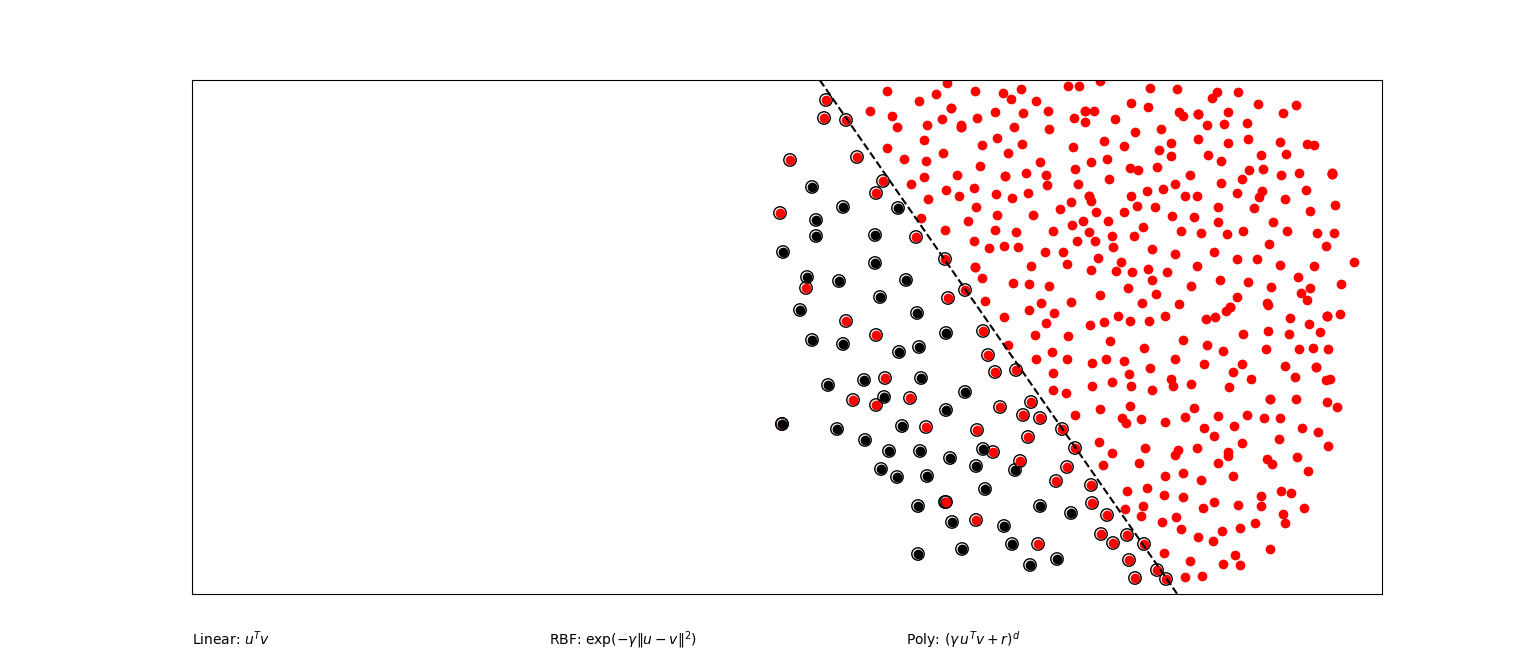
\includegraphics[width=\linewidth]{images/c0.00001.png}
        \caption{SVM avec C=0.00001}
        \label{fig:c00001}
    \end{subfigure}
    \hfill
    \begin{subfigure}{0.45\linewidth}
        \centering
        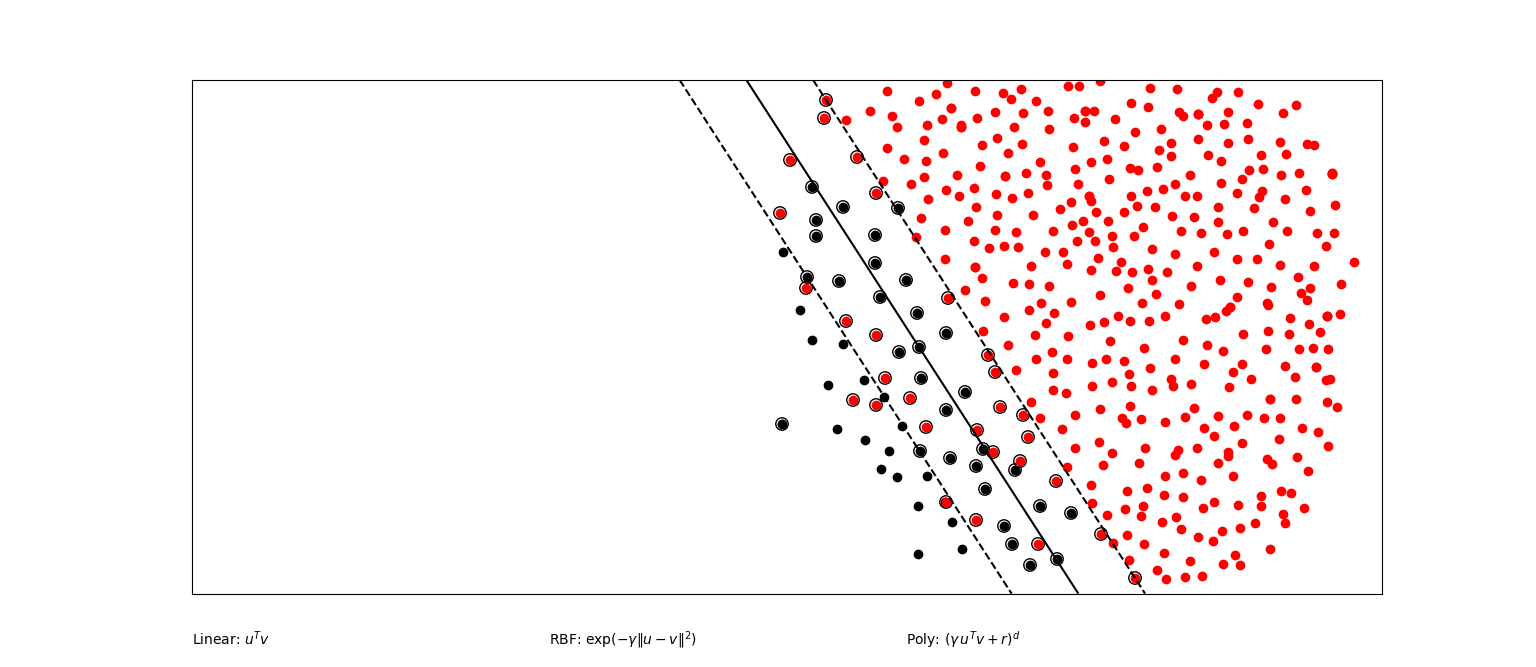
\includegraphics[width=\linewidth]{images/c1.png}
        \caption{SVM avec C=1}
        \label{fig:c1}
    \end{subfigure}

    \vspace{0.5cm} % espace entre la première et la deuxième ligne

    \begin{subfigure}{0.45\linewidth}
        \centering
        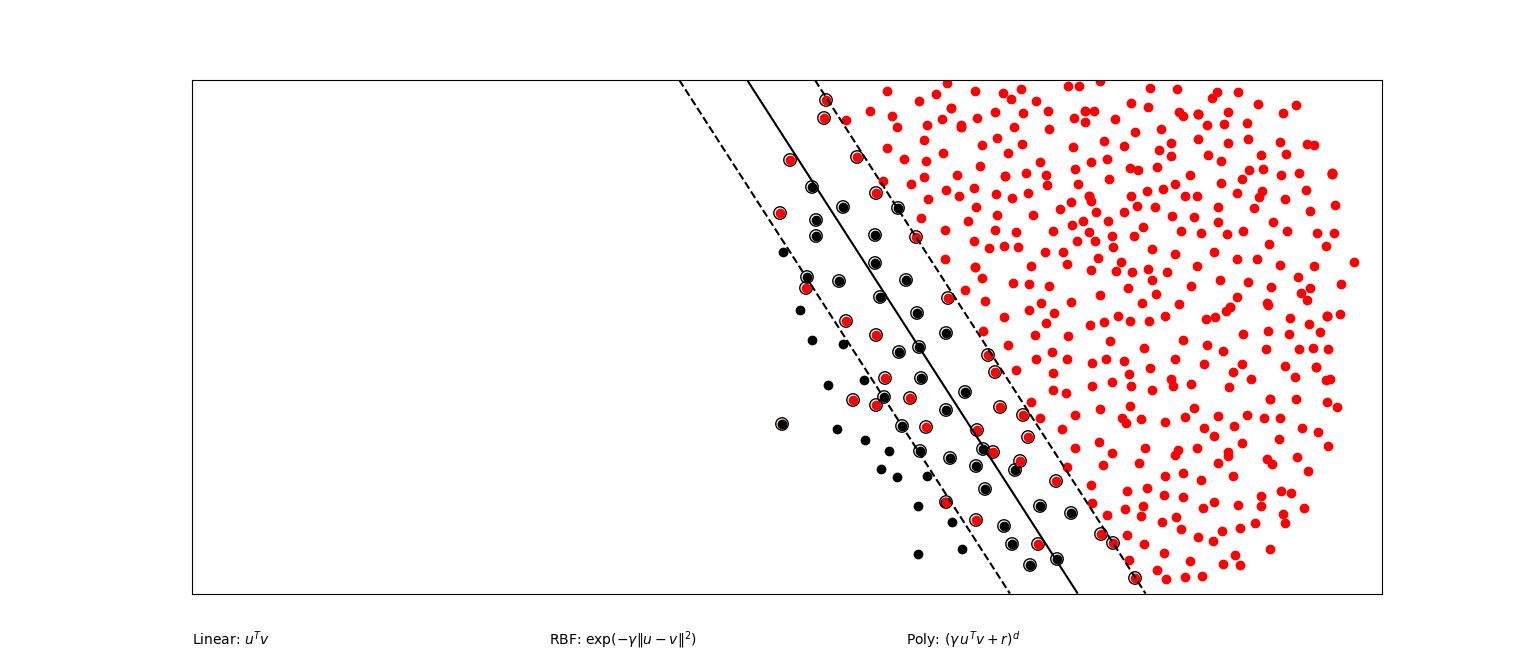
\includegraphics[width=\linewidth]{images/c0.01.png}
        \caption{SVM avec C=0.01}
        \label{fig:c001}
    \end{subfigure}
    \hfill
    \begin{subfigure}{0.45\linewidth}
        \centering
        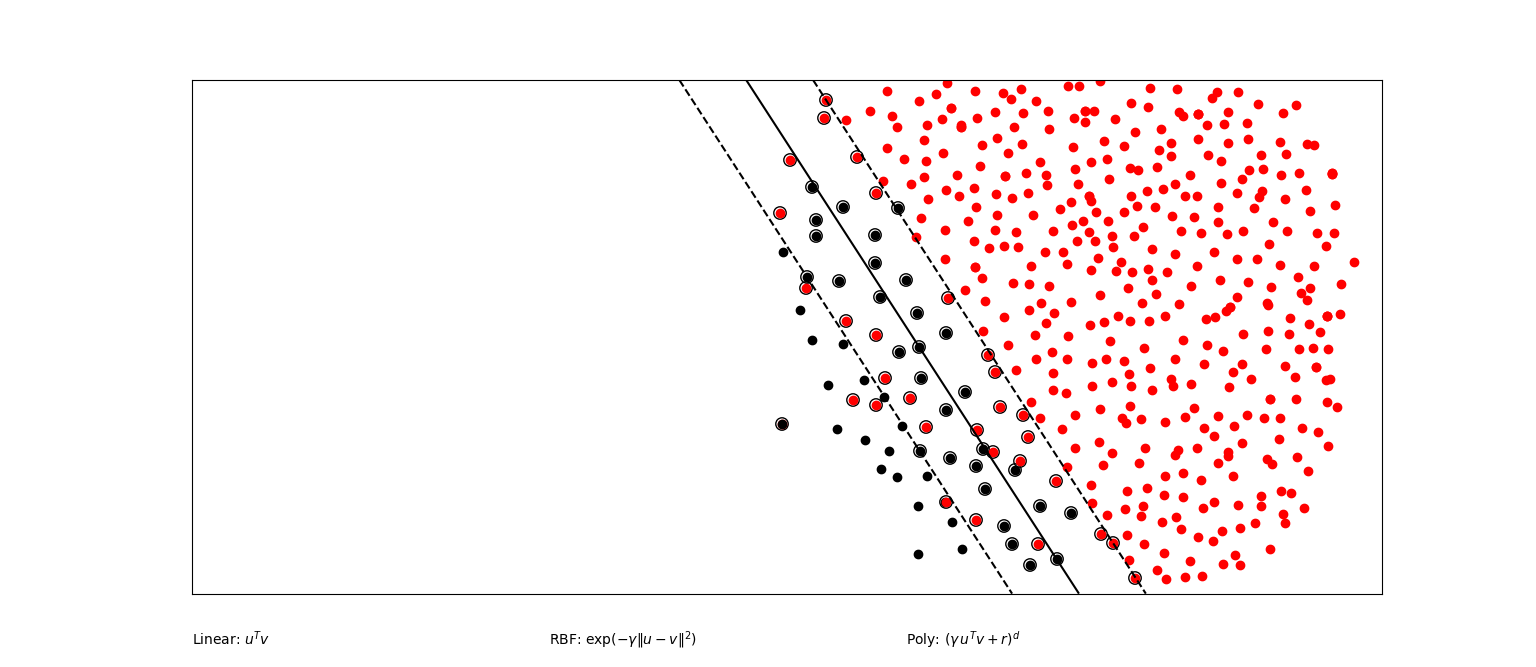
\includegraphics[width=\linewidth]{images/c0.1.png}
        \caption{SVM avec C=0.1}
        \label{fig:c01}
    \end{subfigure}
    
    \caption{Ensemble des résultats regroupés}
    \label{fig:all_results}
\end{figure}

\subsubsection*{Interprétation du paramètre de régularisation \textit{C} :}

Lorsque le paramètre de régularisation est fixé à $C = 1$, le SVM impose une séparation stricte entre les classes. Il cherche à minimiser les erreurs de classification, ce qui se traduit par une marge étroite et une frontière de décision bien définie. Ce réglage accorde une grande importance aux points mal classés, ce qui peut conduire à un surajustement, notamment si les données sont bruitées ou déséquilibrées.

Avec une valeur plus faible, comme $C = 0.1$, le modèle devient plus souple. Il accepte quelques erreurs pour élargir la marge, ce qui améliore la capacité de généralisation. Cependant, certains points proches de la frontière, en particulier ceux de la classe minoritaire, peuvent être mal classés.

En diminuant encore à $C = 0.01$, le SVM tolère davantage d’erreurs. La frontière devient moins précise et la marge s’élargit davantage, au prix d’une perte de précision. Les points minoritaires sont souvent ignorés, ce qui accentue le déséquilibre dans la classification.

Enfin, avec une régularisation très forte comme $C = 0.00001$, le modèle se concentre presque exclusivement sur l’élargissement de la marge. La séparation devient floue et imprécise, avec de nombreux points mal classés, notamment ceux appartenant à la classe minoritaire. Ce comportement illustre une généralisation excessive, où la précision est sacrifiée au profit d’une marge très large.





\section{Classification des visages}
Dans cette section, nous allons travailler sur un problème de classification de visages en
 utilisant le jeu de données Labeled Faces in the Wild (LFW). Ce jeu de données est accessible
 à l’adresse suivante : http://vis-www.cs.umass.edu/lfw/lfw-funneled.tgz.
 
\subsection{Influence du paramètre de régularisation C sur la prédiction}

Nous avons commencé par charger l'ensemble des données LFW en utilisant la fonction \texttt{fetch\_lfw\_people} de \textsc{scikit-learn}, ensuite nous avons sélectionné deux individus dans l'ensemble des données  "Tony Blair" et "Colin Powell" et  nous avons filtré les images pour ne conserver que celles de ces deux personnes.\\

\begin{lstlisting}
lfw_people = fetch_lfw_people(min_faces_per_person=70, resize=0.4,
                              color=True, funneled=False, slice_=None,
                              download_if_missing=True)


# Inspecter les tableaux d'images pour en connaître les dimensions (pour le trace)

images = lfw_people.images
n_samples, h, w, n_colors = images.shape

# L'etiquette a predire est l'identifiant de la personne

target_names = lfw_people.target_names.tolist()
names = ['Tony Blair', 'Colin Powell']
idx0 = (lfw_people.target == target_names.index(names[0]))
idx1 = (lfw_people.target == target_names.index(names[1]))
images = np.r_[images[idx0], images[idx1]]
n_samples = images.shape[0]
y = np.r_[np.zeros(np.sum(idx0)), np.ones(np.sum(idx1))].astype(int)
plot_gallery(images, np.arange(12))
plt.show()
\end{lstlisting}

 Nous avons ensuite extrait les étiquettes pour chaque classe (0 pour Tony Blair
 et 1 pour Colin Powell) et préparé les données pour l’entraînement et les tests.\\
 la figure suivante montre donc l’échantillon des données pour visualiser les images de Tony Blair et Colin Powell.
 
 \begin{figure}[H]
     \centering
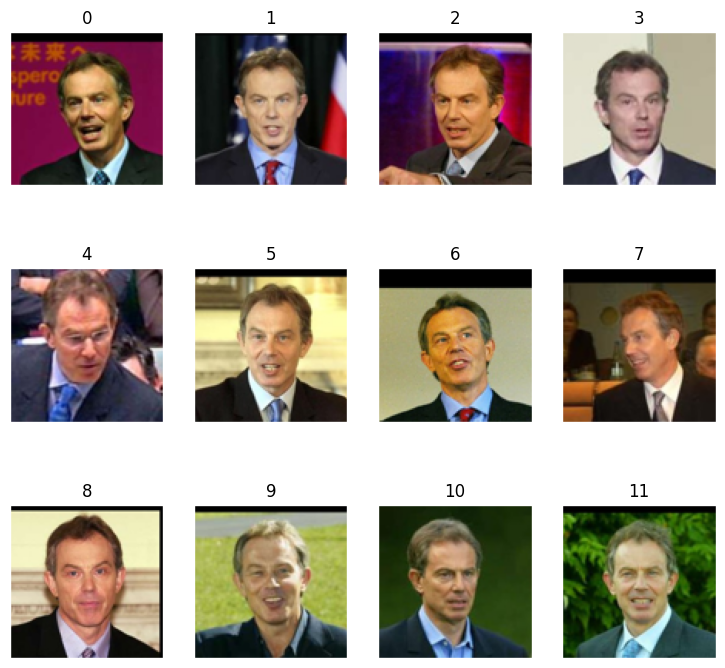
\includegraphics[width=0.9\linewidth]{images/faces.png}
     \caption{}
     \label{fig:placeholder}
 \end{figure}
 Nous avons transformé les images brutes en vecteurs numériques exploitables par le classifieur, soit en niveaux de gris (moins de dimensions), soit en couleur (plus de dimensions). \\
 Avant de procéder à l’entraînement, nous normalisons les caractéristiques pour qu’elles aient
 une moyenne nulle et un écart-type de un. Cela aide le modèle à converger plus rapidement.
 
 \begin{lstlisting}
X = (np.mean(images, axis=3)).reshape(n_samples,-1)
X-= np.mean(X, axis=0)
X /= np.std(X, axis=0)
 \end{lstlisting}
 
\textbf{ Séparation des Données d’Entraînement et de Test\\}
Les données ont été divisées en un ensemble d’entraînement (50\%) et un ensemble de test (50\%) à l’aide d’une permutation aléatoire. 

\begin{lstlisting}
indices = np.random.permutation(X.shape[0])
train_idx, test_idx = indices[:X.shape[0] // 2], indices[X.shape[0] // 2:]
X_train, X_test = X[train_idx, :], X[test_idx, :]
y_train, y_test = y[train_idx], y[test_idx]
images_train, images_test = images[
    train_idx, :, :, :], images[test_idx, :, :, :]  
\end{lstlisting}
\textbf{ Ajustement du Modèle SVM avec Noyau Linéaire\\}
 Nous avons entraîné plusieurs modèles SVM en utilisant un noyau linéaire avec
 différentes valeurs du paramètre de régularisation C (allant de $10^{-5}$ à $10^5$). Le but
 était de déterminer la meilleure valeur de C en fonction de la précision sur l’ensemble
 de test.
\begin{lstlisting}
print("--- Linear kernel ---")
print("Fitting the classifier to the training set")
t0 = time()
# fit a classifier (linear) and test all the Cs
Cs = 10. ** np.arange(-5, 6)
scores = []
for C in Cs:
    # 
    clf = SVC(kernel='linear', C=C)
    # Entraîner le modele sur l'ensemble d'entraînement
    clf.fit(X_train, y_train)
    # Prédire les labels sur l'ensemble de test
    y_pred = clf.predict(X_test)
    
    # Calculer le score (accuracy) et l'ajouter à la liste des scores
    score = accuracy_score(y_test, y_pred)
    scores.append(score)   
\end{lstlisting}
Ensuite, nous avons identifié la meilleure valeur de C et affiché la courbe des scores en fonction de C.
\begin{figure}[H]
    \centering
    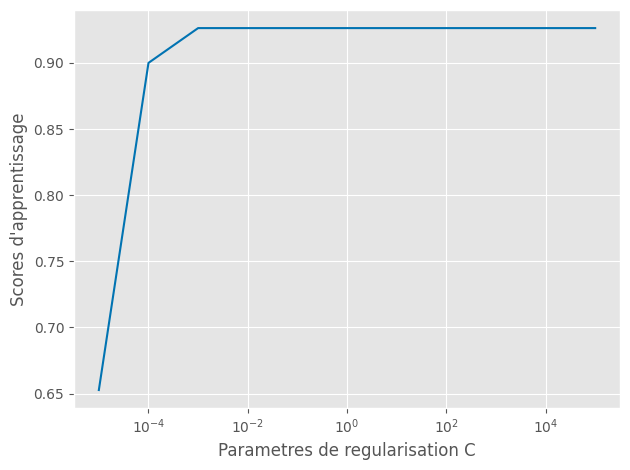
\includegraphics[width=1\linewidth]{images/paramC.png}
    \caption{Parametre C}
    \label{fig:placeholder}
\end{figure}
Ces résultats indiquent que la meilleure valeur de C est 0.001 où le modèle atteint un score d'environ 94\%, avec une plus faible valeur de C la précision est d'environ 65\% mais elle augmente rapidement jusqu’à ce que C atteigne la valeur 0.001 et après la précision devient stable. Cela montre que cette valeur de C fournit le bon équilibre entre généralisation et performance pour cette tâche de reconnaissance de visages.
\subsection{Prédiction des étiquettes des images avec le meilleur classificateur}
\begin{lstlisting}
print("Predicting the people names on the testing set")
t0 = time()

# Utiliser la meilleure valeur de C pour prédire
best_clf = SVC(kernel='linear', C=Cs[ind])
best_clf.fit(X_train, y_train)
y_pred_best = best_clf.predict(X_test)

# Afficher le score final avec le meilleur C
final_score = accuracy_score(y_test, y_pred_best)
print("Final accuracy with best C: {:.2f}".format(final_score))
clf =  best_clf
t0 = time()
y_pred = clf.predict(X_test)  # Prédiction des labels

print("done in %0.3fs" % (time() - t0))
# The chance level is the accuracy that will be reached when constantly predicting the majority class.
print("Chance level : %s" % max(np.mean(y), 1. - np.mean(y)))
print("Accuracy : %s" % clf.score(X_test, y_test))
\end{lstlisting}
\begin{itemize}
    \item Temps d’exécution : 0.162s
    \item Niveau de chance : 62.1\%
    \item Préccision du modéle : 92\%
\end{itemize}

\subsection{Évaluation qualitative des prédictions}

Nous avons généré des titres comparant la prédiction du modèle à la vérité terrain,
 et nous avons affiché une galerie d’images pour une évaluation visuelle des résultats.
\begin{lstlisting}
prediction_titles = [title(y_pred[i], y_test[i], names)
                     for i in range(y_pred.shape[0])]

plot_gallery(images_test, prediction_titles)
plt.show()
\end{lstlisting}

\begin{figure}[H]
    \centering
    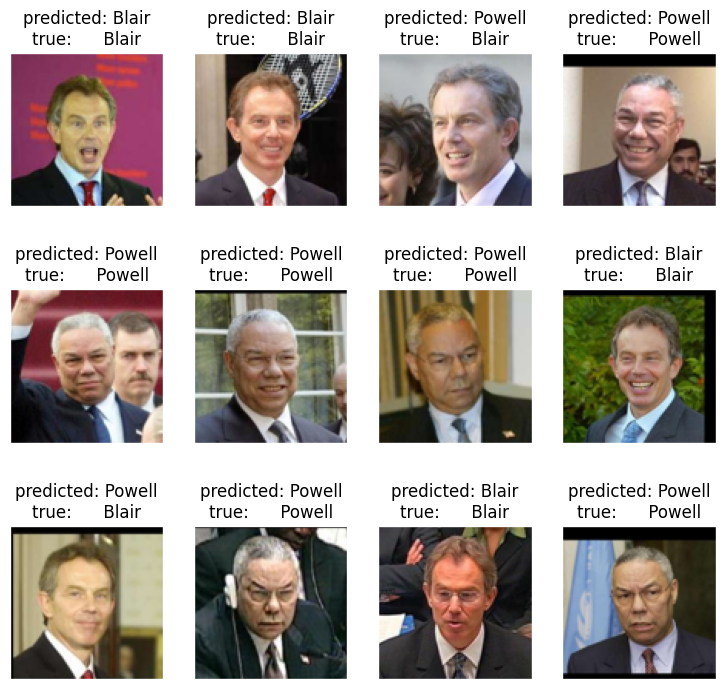
\includegraphics[width=0.9\linewidth]{images/predvis.png}
    \caption{Classification des Visages}
    \label{fig:placeholder}
\end{figure}
Ces images comparent les vraies étiquettes avec les prédictions du modèle.\\
- Lorsque l’on observe les cas « predicted : Powell, true : Powell », le modèle parvient à identifier correctement Powell, ce qui traduit une bonne capacité de reconnaissance. De même, les images « predicted : Blair, true : Blair » confirment la justesse des prédictions pour Blair et soulignent la performance du modèle.\\
- En revanche, certaines erreurs apparaissent, par exemple lorsque Powell est prédit par Blair ou inversement.
 Ces erreurs peuvent être liées à une généralisation insuffisante du modèle ou bien à des ressemblances entre les visages. Pour au mieux comprendre cet enjeu, nous allons observer la figure suivante :
\begin{figure}[H]
    \centering
    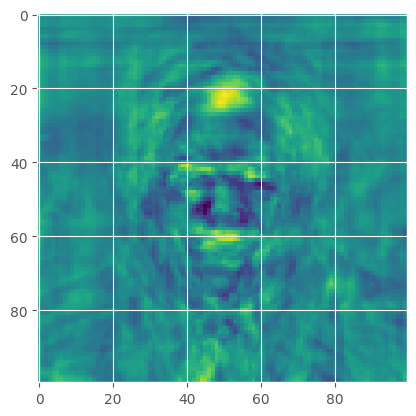
\includegraphics[width=0.9\linewidth]{images/predic.png}
    \caption{ Classification de visages}
    \label{fig:placeholder}
\end{figure}
Cette image représente les coefficients du modèle SVM appris à partir du jeu de données, visualisés sous forme de matrice semblable à une image. Chaque pixel traduit ainsi l'importance d'une caractéristique (un pixel du visage) dans la décision de classification.
\begin{itemize}
    \item Les zones lumineuses (jaune et vert clair) mettent en évidence les régions qui influencent fortement la prédiction, en particulier autour des yeux, du nez et de la bouche.
    \item Les zones sombres (bleu et noir) correspondent aux parties du visage ayant peu ou pas d’impact sur la décision.
\end{itemize}
On constate donc que le modèle se focalise sur certaines zones clés du visage pour distinguer les classes, ce qui correspond aux traits distinctifs généralement utilisés par l'humain dans la reconnaissance faciale.

\subsection{Influence des variables de nuisance}

L’objectif de ce code est de montrer que l’ajout de variables de nuisance 
(bruit) aux données d’apprentissage détériore les performances d’un modèle SVM. 
Nous commençons par entraîner le modèle sur les données initiales, puis nous 
introduisons des variables aléatoires de bruit et comparons les résultats sur 
l’ensemble de test.


\begin{lstlisting}
def run_svm_cv(_X, _y):
    _indices = np.random.permutation(_X.shape[0])
    _train_idx, _test_idx = _indices[:_X.shape[0] // 2], _indices[_X.shape[0] // 2:]
    _X_train, _X_test = _X[_train_idx, :], _X[_test_idx, :]
    _y_train, _y_test = _y[_train_idx], _y[_test_idx]

    # Parametres pour SVM lineaire avec C variant sur une plage logarithmique
    _parameters = {'kernel': ['linear'], 'C': list(np.logspace(-3, 3, 5))}
    _svr = svm.SVC()
    _clf_linear = GridSearchCV(_svr, _parameters)
    _clf_linear.fit(_X_train, _y_train)

    # Calcul des scores sur les donnees d'entraînement et de test
    print('Generalization score for linear kernel: %s, %s \n' %
          (_clf_linear.score(_X_train, _y_train), _clf_linear.score(_X_test, _y_test)))

# Exécution du SVM sur les donnees sans nuisance
print("Score sans variable de nuisance")
run_svm_cv(X, y)

# Ajout des variables de nuisance (bruit)
n_features = X.shape[1]
sigma = 1
# Generation de 300 variables de nuisance avec une distribution gaussienne
noise = sigma * np.random.randn(n_samples, 300)
X_noisy = np.concatenate((X, noise), axis=1)  # Ajout des variables de nuisance aux donnees originales
X_noisy = X_noisy[np.random.permutation(X.shape[0])]  # Permutation aleatoire des donnees pour ne pas biaiser les resultats

# Execution du SVM sur les donnees avec variables de nuisance
print("Score avec variables de nuisance")
run_svm_cv(X_noisy, y)
\end{lstlisting}

L’ajout de variables de nuisance aux données a un impact très négatif sur la performance du modèle SVM. Sans variables de nuisance, le modèle atteint un score de 1.0 sur l’entraînement et 0.91 sur le test, ce qui montre qu’il apprend correctement et généralise bien. En ajoutant 300 variables de nuisance, le score sur l’entraînement reste 1.0, mais celui sur le test chute à 0.54, révélant un fort surapprentissage. Ces variables augmentent la dimension des données sans fournir d’information utile, réduisant considérablement la capacité du modèle à généraliser sur de nouvelles données.


\subsection{Amélioration de la prédiction par réduction de dimension (PCA)}


Nous avons utilisé une réduction de dimension par PCA sur les données bruitées en sélectionnant un nombre ajustable de composantes principales. Nous avons choisi initialement 20 composantes et contrôlé la variance expliquée pour vérifier qu'elles capturent suffisamment d'informations des données.

\begin{lstlisting}
print("Score apres reduction de dimension avec PCA")

n_components = 30 # Nombre de composantes principales (peut etre ajuste)
pca = PCA(n_components=n_components, svd_solver='randomized').fit(X_noisy)

# Transformation des donnees avec PCA
X_noisy_pca = pca.transform(X_noisy)

# On affiche la variance expliquee pour choisir le bon nombre de composantes
explained_variance = np.sum(pca.explained_variance_ratio_)
print(f"Variance expliquee avec {n_components} composantes : {explained_variance:.2\%}")
\end{lstlisting}







Après réduction de dimension avec PCA, nous avons testé différents nombres de composantes principales : \\
- 20 composantes : variance expliquée 67,67\,\%.  \\
- 30 composantes : variance expliquée 73,56\,\%.  \\
- 50 composantes : variance expliquée 80,11\,\% . \\

Ces résultats montrent qu'avec 30 à 50 composantes, une grande partie de l'information originale est conservée tout en réduisant la dimension des données. Le choix de 30 composantes constitue un bon compromis entre conservation de l'information et temps de calcul, permettant au modèle SVM de mieux généraliser et de limiter l'effet des variables de nuisance.





\subsection{ Biais dans le prétraitement}

Dans le script fourni, la normalisation est effectuée sur l’ensemble complet des données
avant de séparer en train et test. Cela crée un biais, car les statistiques de centrage
et de réduction (moyenne et écart-type) intègrent déjà l’information contenue dans le test,
ce qui revient à utiliser indirectement ces données lors de l’apprentissage.

La correction consiste à appliquer la normalisation uniquement sur l’ensemble
d’entraînement, puis à utiliser les mêmes paramètres pour transformer le test :

\begin{lstlisting}
    
from sklearn.preprocessing import StandardScaler

scaler=StandardScaler()
X_train=scaler.fit_transform(X_train) #fit uniquement sur le train
X_test=scaler.transform(X_test)#appliquer au test

\end{lstlisting}



Ainsi, aucune information du test n’est utilisée avant l’évaluation, ce qui évite la fuite
de données et garantit une estimation plus fiable des performances du modèle.



\section{Conclusion}
%\addcontentsline{toc}{chapter}{Conclusion}


Ce TP a montré que les SVM constituent des méthodes de classification
robustes et efficaces, à condition de bien choisir les hyperparamètres et le
noyau adaptés aux données. Nous avons observé l’impact direct du paramètre
de régularisation \(C\), l’intérêt des noyaux non linéaires pour traiter des
données complexes, ainsi que les limites introduites par le bruit et les variables
de nuisance. L’utilisation de techniques comme la PCA s’est révélée essentielle
pour améliorer la généralisation. Ce travail nous a ainsi permis de relier la
théorie des SVM à leur mise en pratique sur des données réelles.

 
\end{document}
